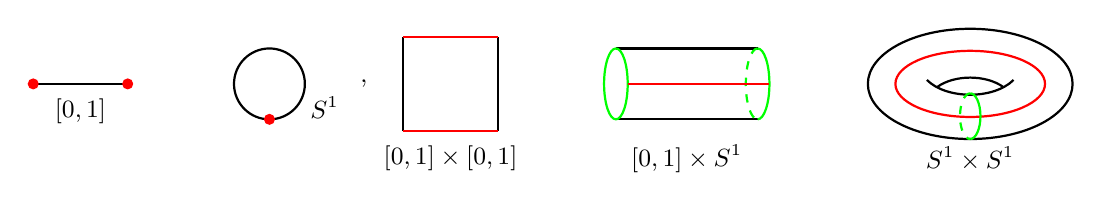
\begin{tikzpicture}[line width=0.8pt, every node/.style={font=\small}]
  % [0,1] -> S^1
  \draw (0,0) -- (1.2,0);
  \fill[red] (0,0) circle (2pt) (1.2,0) circle (2pt);
  \node at (0.6,-0.35) {$[0,1]$};
  \node at (1.90,0) {$\rightsquigarrow$};
  \draw (3.0,0) circle (0.45);
  \fill[red] (3.0,-0.45) circle (2pt);
  \node at (3.7,-0.3) {$S^1$};
  \node at (4.2,0) {,};
  % square -> cylinder -> torus
  \draw (4.7,-0.6) -- (4.7,0.6) (5.9,-0.6) -- (5.9,0.6);
  \draw[red] (4.7,-0.6) -- (5.9,-0.6) (4.7,0.6) -- (5.9,0.6);
  \node at (5.3,-0.95) {$[0,1]\times[0,1]$};
  \node at (6.60,0) {$\rightsquigarrow$};
  \begin{scope}[shift={(8.3,0)}]
    \draw (-0.9,0.45) -- (0.9,0.45) (-0.9,-0.45) -- (0.9,-0.45);
    \draw[green] (-0.9,0) ellipse (0.15 and 0.45);
    \draw[green] (0.9,-0.45) arc[start angle=-90, end angle=90, x radius=0.15, y radius=0.45];
    \draw[green, dashed] (0.9,0.45) arc[start angle=90, end angle=270, x radius=0.15, y radius=0.45];
    \draw[red] (-0.75,0) -- (1.05,0);
    \node at (0,-0.95) {$[0,1]\times S^1$};
  \end{scope}
  \node at (10.00,0) {$\rightsquigarrow$};
  \begin{scope}[shift={(11.9,0)}]
    \draw (0,0) ellipse (1.3 and 0.7);
    \draw (-0.55,0.05) .. controls (-0.3,-0.2) and (0.3,-0.2) .. (0.55,0.05);
    \draw (-0.42,-0.04) .. controls (-0.2,0.12) and (0.2,0.12) .. (0.42,-0.04);
    \draw[red] (0,0) ellipse (0.95 and 0.42);
    \draw[green] (0,-0.7) arc[start angle=-90, end angle=90, x radius=0.13, y radius=0.29];
    \draw[green, dashed] (0,-0.12) arc[start angle=90, end angle=270, x radius=0.13, y radius=0.29];
    \node at (0,-0.95) {$S^1\times S^1$};
  \end{scope}
\end{tikzpicture}
